In proposed SIMEX development project, we focus to investigate the possible
route for experimental realization of laser plasma accelerator based coherent
light source (FELs)\cite{Emma2004}. Since the conventional accelerator has the limit of the
gradient due to the structure surface field limit, the best gradient achieved
now is less than 100MeV/m. Laser plasma accelerator
(LPA)\cite{Leemans2006,Esarey2009,Tajima1979} will be the next
generation accelerator facilities with the ultrahigh gradient which will reach
100GeV/m. Due to the ultrahigh gradient of LPA, the accelerator facility will
be miniaturized greatly.

Here we are employing an extension of SIMEX platform to enable simulation of
LWFA based coherent light sources (FELs) by coupling a particle-in-cell (PIC)
code (PIConGPU)\cite{Bussmann2013} that describes the LWFA to a FEL simulation
code (GENESIS)\cite{genesis_online}.

Proposed Setup for SIMEX:

Our proposed setup is shown in Fig.~1; starting from electron beam generation
from a laser plasma source to the generation of femtosecond and/or attosecond
EUV/XUV pulse from the radiation undulator at endpoint. In this scheme an
intense.
%
\begin{figure}[ht]
  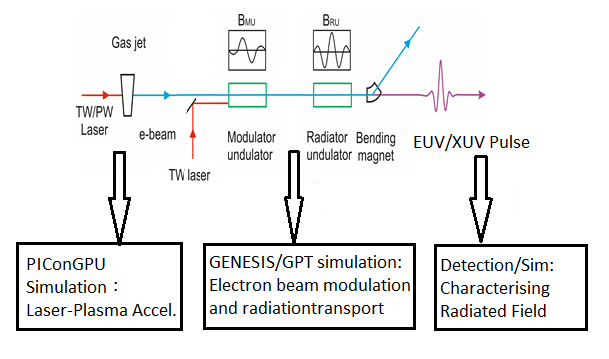
\includegraphics[width=5.4165in,height=2.7374in]{figures/lwfafel-img001.png}
  \caption{Scheme of the proposed setup}
  \label{lwfa-fig1}
\end{figure}
%
(TW/PW power) laser is focused on gas jet/ gas filled capillary for producing a
relativistic electron beam. Initial energy spread of the electron beam of a
LPAs (1-5\%) is typically much larger than that of a LINAC (about 0.05 \%), so
reduction of the slice energy spread is necessary. The electron beam is sent
through a modulator undulator (MU) together with a TW-power laser beam, where
the interaction between the electrons, the magnetic field of the undulator and
the electromagnetic field of the laser introduces a periodic energy modulation
of the electrons. This energy modulation leads to the formation of nanobunches
(ultrashort electron layers). The nanobunched electron beam then passes through
a radiator undulator (RU) consisting of a single or a few periods and creates
EUV/XUV pulses.


We proceed in this SIMEX development for LPA-FEL following two parallel paths:
\begin{enumerate}
  \item Development of SIMEX setup for LPA-FEL by combining PIConGPU and GENESIS,
  \item Utilisation of experimentally achieved high quality electron beam as an
    input to FEL simulation codes GPT \cite{gpt_online} or
    GENESIS\cite{genesis_online}, for investigation of coherent
    radiation generation.
\end{enumerate}


\begin{figure}
  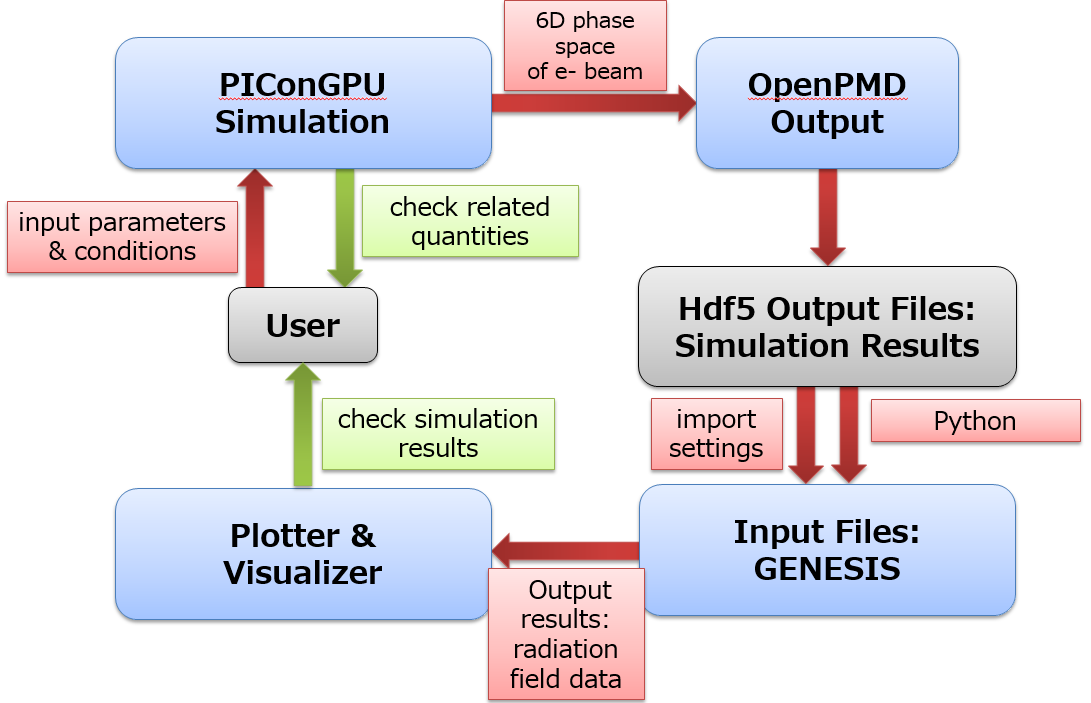
\includegraphics[width=5.9425in,height=4.1882in]{figures/lwfafel-img002.png}
  \caption{Layout for Simulation Setup}
  \label{lwfa-fig2}
\end{figure}

\begin{enumerate}
\item Laser-plasma accelerator based single-cycle attosecond undulator source
(in collaboration with T. Zoltan and Prof. Hebling, Pecs University Hungary)
\end{enumerate}


The following figure shows example results which are discussed in detail in
Ref.~\cite{Tibai2017}

\begin{figure}
  \centering{%
    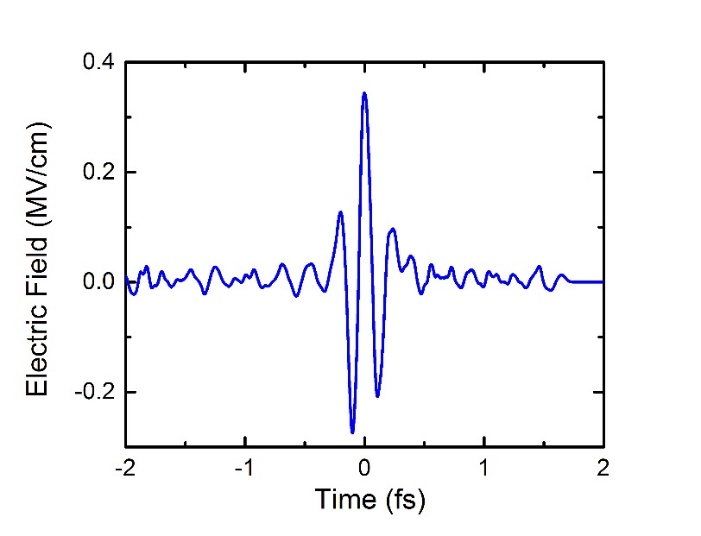
\includegraphics[width=2.7016in,height=2.1583in]{figures/lwfafel-img003.jpg}
    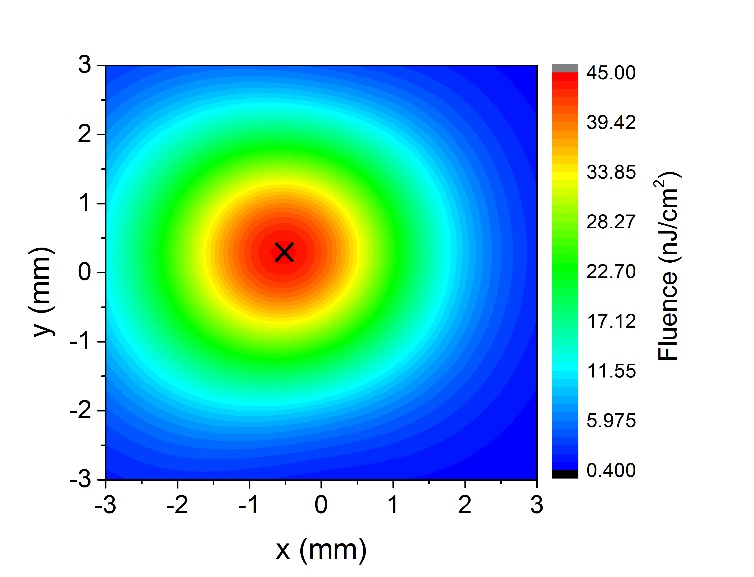
\includegraphics[width=3.0083in,height=2.352in]{figures/lwfafel-img004.jpg}
  }
  \caption{GPT Simulation Results: CEP-controlled EUV waveforms (left) and its spatial beam
  profile (right).}
\end{figure}

Figure shown here, \ displays the simulated waveform of the generated attosecond
pulse and the beam profile at 60 nm radiation wavelength. The location of the
waveform in fig (a) is shown in figure (b) marked with a symbol x. In other
wavelengths the shape of the attosecond pulses are nearly identical with the
shape shown in fig (a) so these pulses are CEP controlled too.

%References

%[1] P. Emma, K. Bane, M. Cornacchia, Z. Huang, H. Schlarb, G. Stupakov, and D.
%Walz, Phys. Rev. Lett. 92, 074801 (2004)

%[2] W. P. Leemans et al, Nat. Phys. 2, 696 (2006)

%[3] E. Esarey et al, Rev. Mod. Phys. 81, 1229 (2009)

%[4] T. Tajima and J. M. Dawson, Phys. Rev. Lett. 43, 267 (1979).

%[5] ~M. Bussmann et al,~Proceedings SC13: International Conference for High
%Performance Computing, Networking, Storage and Analysis~\textbf{5-1}, 2013.

%[6] GPT: online at http://www.pulsar.nl/gpt

%[7] GENESIS: online at http://genesis.web.psi.ch/
